\chapter{Grundlegendes}
\label{cha:grundlegendes}
% 3 Seiten

\section{Definition}

eine teil aus dem Bereich der Maschine Learning-Algorithmen
zum errechnen vieler Repräsentationen und Features durch die Berechnung nicht-linearer Informationen
supervised und unsupervised feature extracaction


Deep Learning kommt aus dem Maschine Learning und befasst sich mit dem maschninellen lernen von vielschichtigen netzten, wie zum Beispiel vielschichtigen neuronalen Netzen oder Deep Belive Netzten.

\section{Entstehung}

Der Backpropagation Algorithmus wurde in den 1970ern und 1980ern mehrmals erfunden?! (Werbos, Amari?, Parker, LeCun, Rumelhart, ..)

Backpropagation sah vielversprechend aus, aber in den 1990ern hat er an Bedeutung verlohren da die vielen hidden layer nicht trainiert werden konnten (rechenpower außer bei time-delay und convolutional nets) + hat nicht für netzwerke mit feedback funktioniert

negativ: benötigt gelabelte daten, ungelabelt stehen viel viel viel mehr zur verfügung
negativ: zeit für lernen skaliert schlecht
negativ: langsam bei netzwerken mit mehreren hidden layern
negativ: bleibt oft in lokalen minima hängen, besonders bei vielschichtigen netzten!

frage ob deep-nets wirklich besser als wenigschichtige Netzte sind

supervised gegen unsupervised: ist unsupervised lerning nur ein behelf weil zu wenig gelabelte daten vorhanden sind oder ist eigentlich jedes lernen unsupervised und es scheitert nur an der Rechenleistung?

wie viel wissen sollten wir vorab in die daten stecken (kantenerkennung etc.), ist das netzt mit entsprechender Rechenpower nicht immer besser?

backpropagation-limitierungen mit notwendigkeit für gelabelte daten aufheben: mit unsupervised-learning beheben, gewichte anpassen wie in backpropagation gut, aber versuchen das eingangsbild aus den parametern wiederherzustellen, damit lernt das netz automatisch in unterster schicht wie bilder aussehen bevor es bilder identifiziert




backpropagation invented several times in the 1970 and 1980

heute besonders durch die vermehrte Speicherung von unkategorisierten Daten durch Unternehmen wie Google, Facebook und co. vermehrt unsupervised algorithmen und massiv viel rechenpower
vorab rechenpower und datenmänge gewinnt gegen coolen algorithmus

\section{Hürden}

rotation, mutation der Natur
\todo[inline]{beschreibt dass es früher probleme gab, linzer in beteiligung: http://www.kurzweilai.net/how-bio-inspired-deep-learning-keeps-winning-competitions}

\section{Neuronale netze}

\begin{figure}
	\centering
	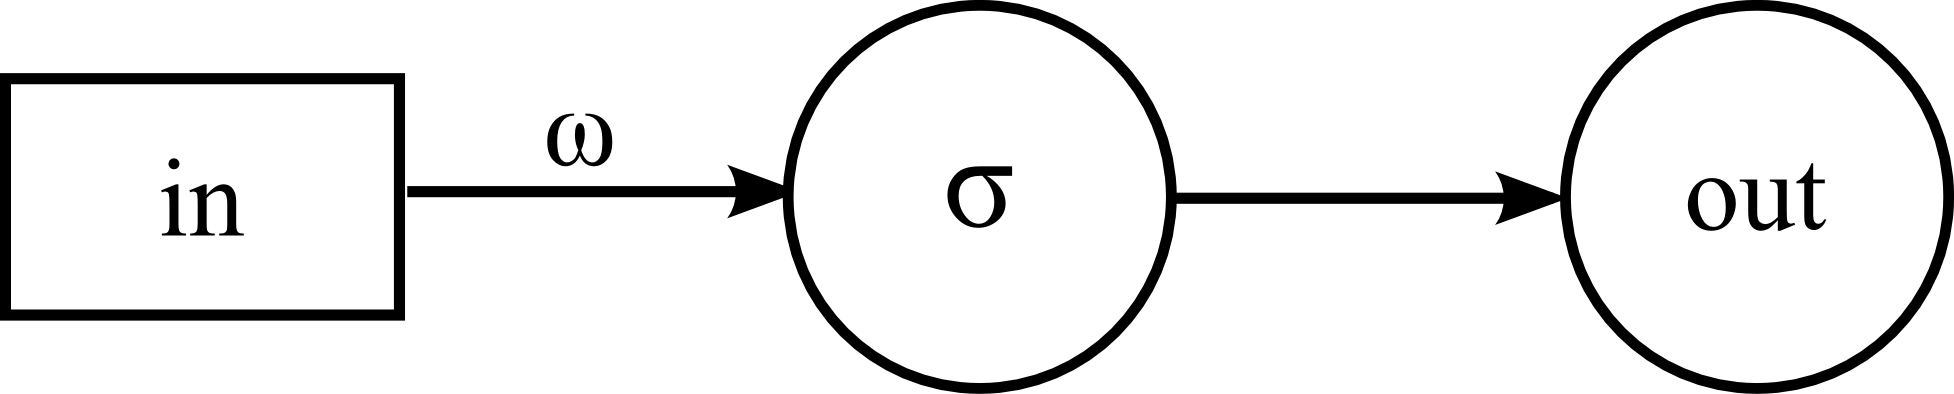
\includegraphics[scale=1]{images/neuron.png}
	\caption{Neuron}
	\label{fig:neuron}
\end{figure}

Neuronale Netze sind Strukturen aus der Technik, die dem Nervensystem von Lebewesen ähneln. Es sind Modelle, die Eingangsdaten über Neuronen gewichtet kombinieren und daraus einen Ausgang errechnen. Neuronale Netze sind in der Technik zur Vereinfachung meist in mehreren Schichten aufgebaut.

Abbildung \ref{fig:neuron} zeigt ein einfaches Neuron mit einem Eingang. Ein Eingang wird mit dem Gewicht multipliziert um dann anhand der Übertragungsfunktion den Ausgang zu berechnen. Als Übertragungsfunktion dient meist die Sigmoid-Funktion, welche sich einfach differenzieren lässt und sich daher besonders gut eignet. Der Ausgang $out$ dieses Neurons ergibt sich somit aus der dem Eingang $in$ multipliziert mit dem Gewicht $\omega$ in der Sigmoid-Funktion $\sigma$.
$$out = \sigma(\omega * in)$$

\begin{figure}
	\centering
	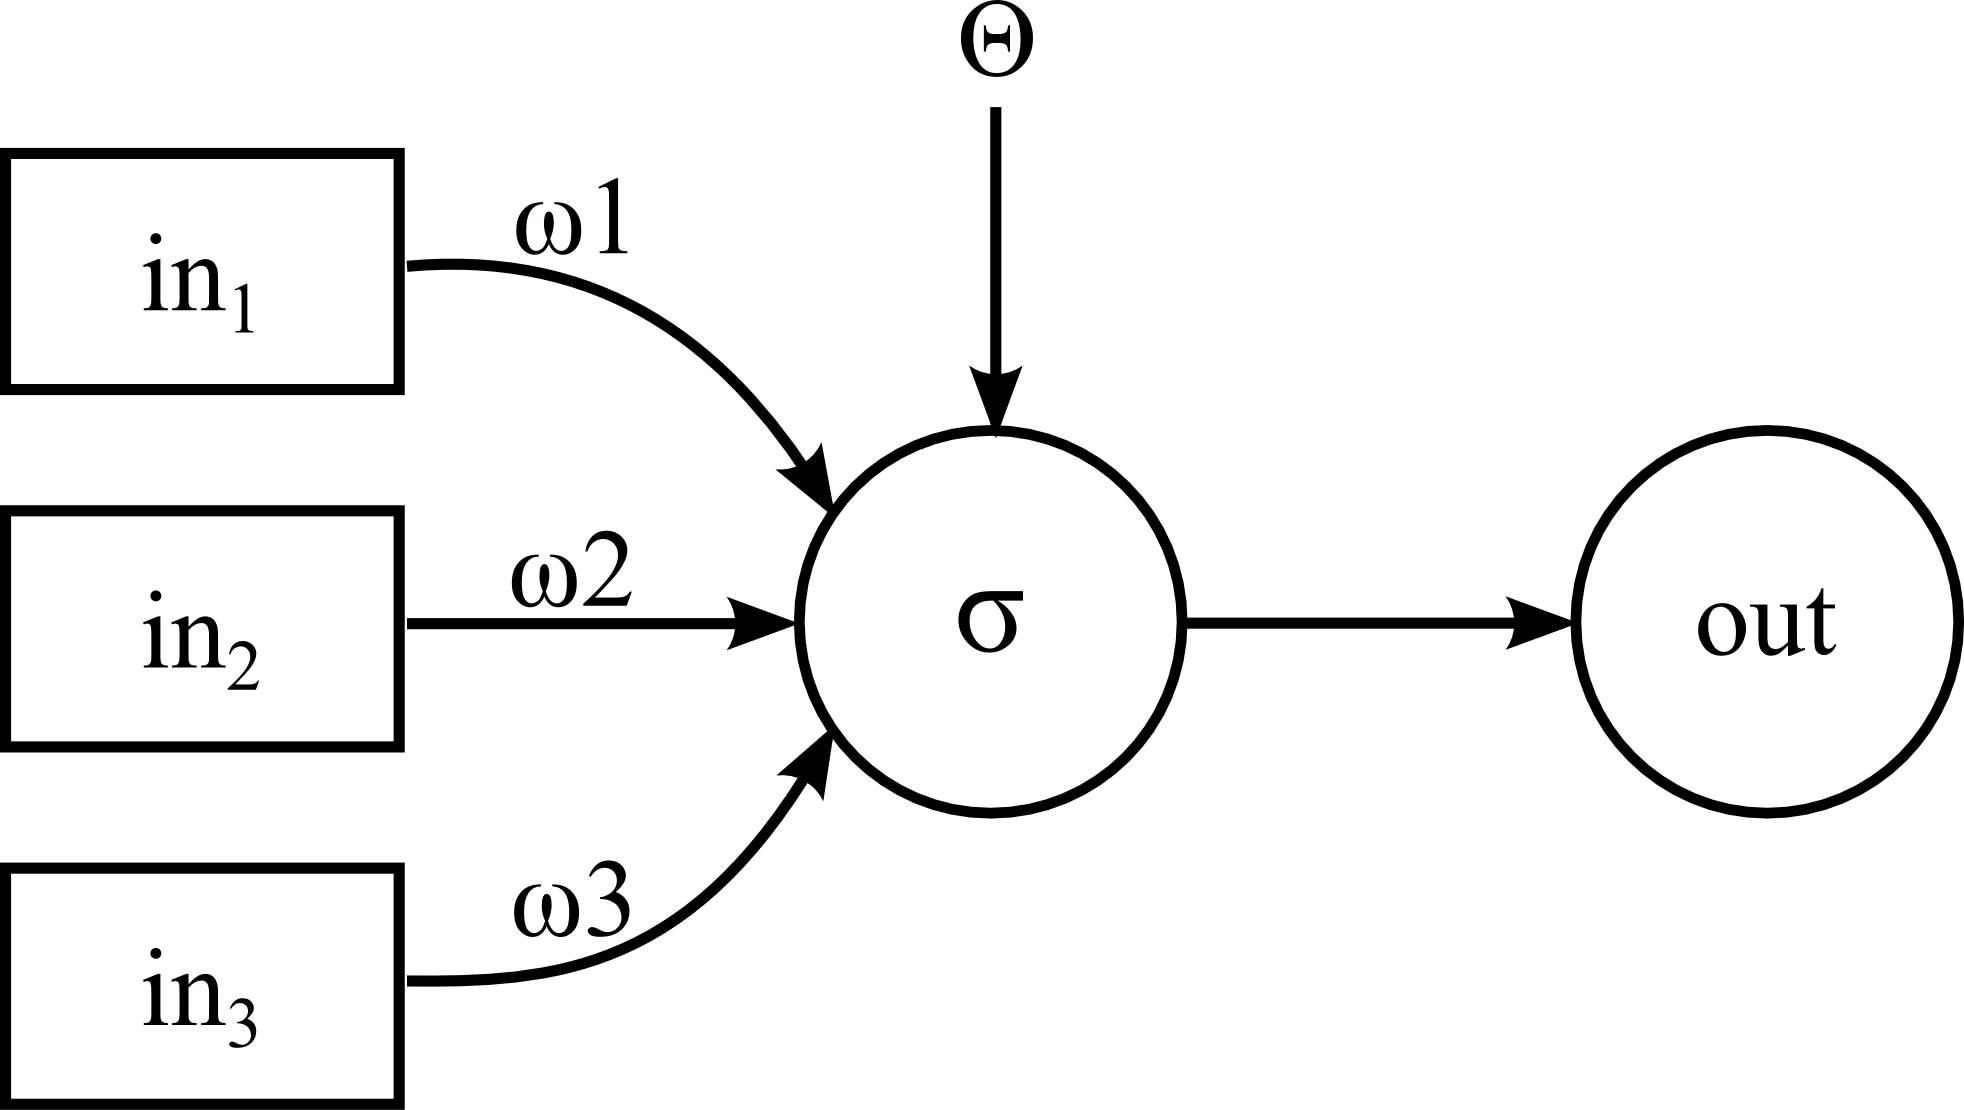
\includegraphics[scale=1]{images/neuron-multiple-inputs.png}
	\caption{Neuron mit mehreren Eingängen}
	\label{fig:neuron-multiple-inputs}
\end{figure}

Ein Neuron hat in der Regel, wie in Abbildung \ref{fig:neuron-multiple-inputs} zu sehen, mehrere Eingänge. Außerdem wird noch ein Bias-Wert $\theta$ für die Sigmoid-Funktion hinzugefügt. Der Ausgang dieses Neurons kann somit wie folgt berechnet werden:
$$out = \sigma(\omega_1*in_1 + \omega_2*in_2 + \omega_3*in_3 + \theta)$$

\begin{figure}
	\centering
	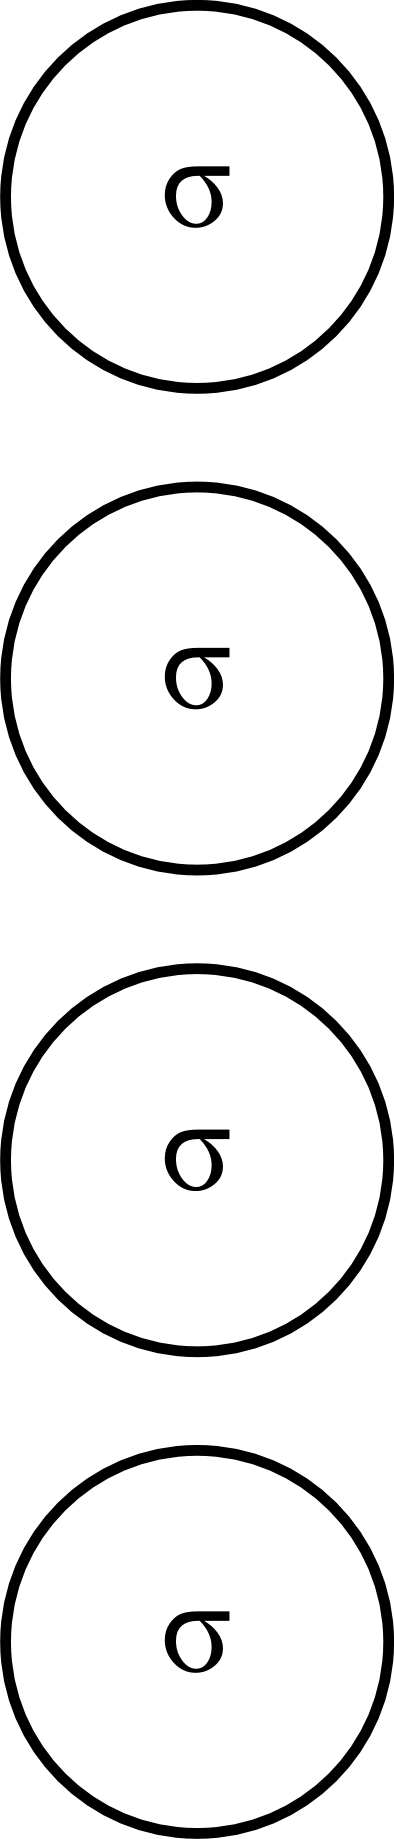
\includegraphics[scale=1]{images/neuron-layer.png}
	\caption{Layer von Neuronen}
	\label{fig:neuron-layer}
\end{figure}

\begin{figure}
\centering
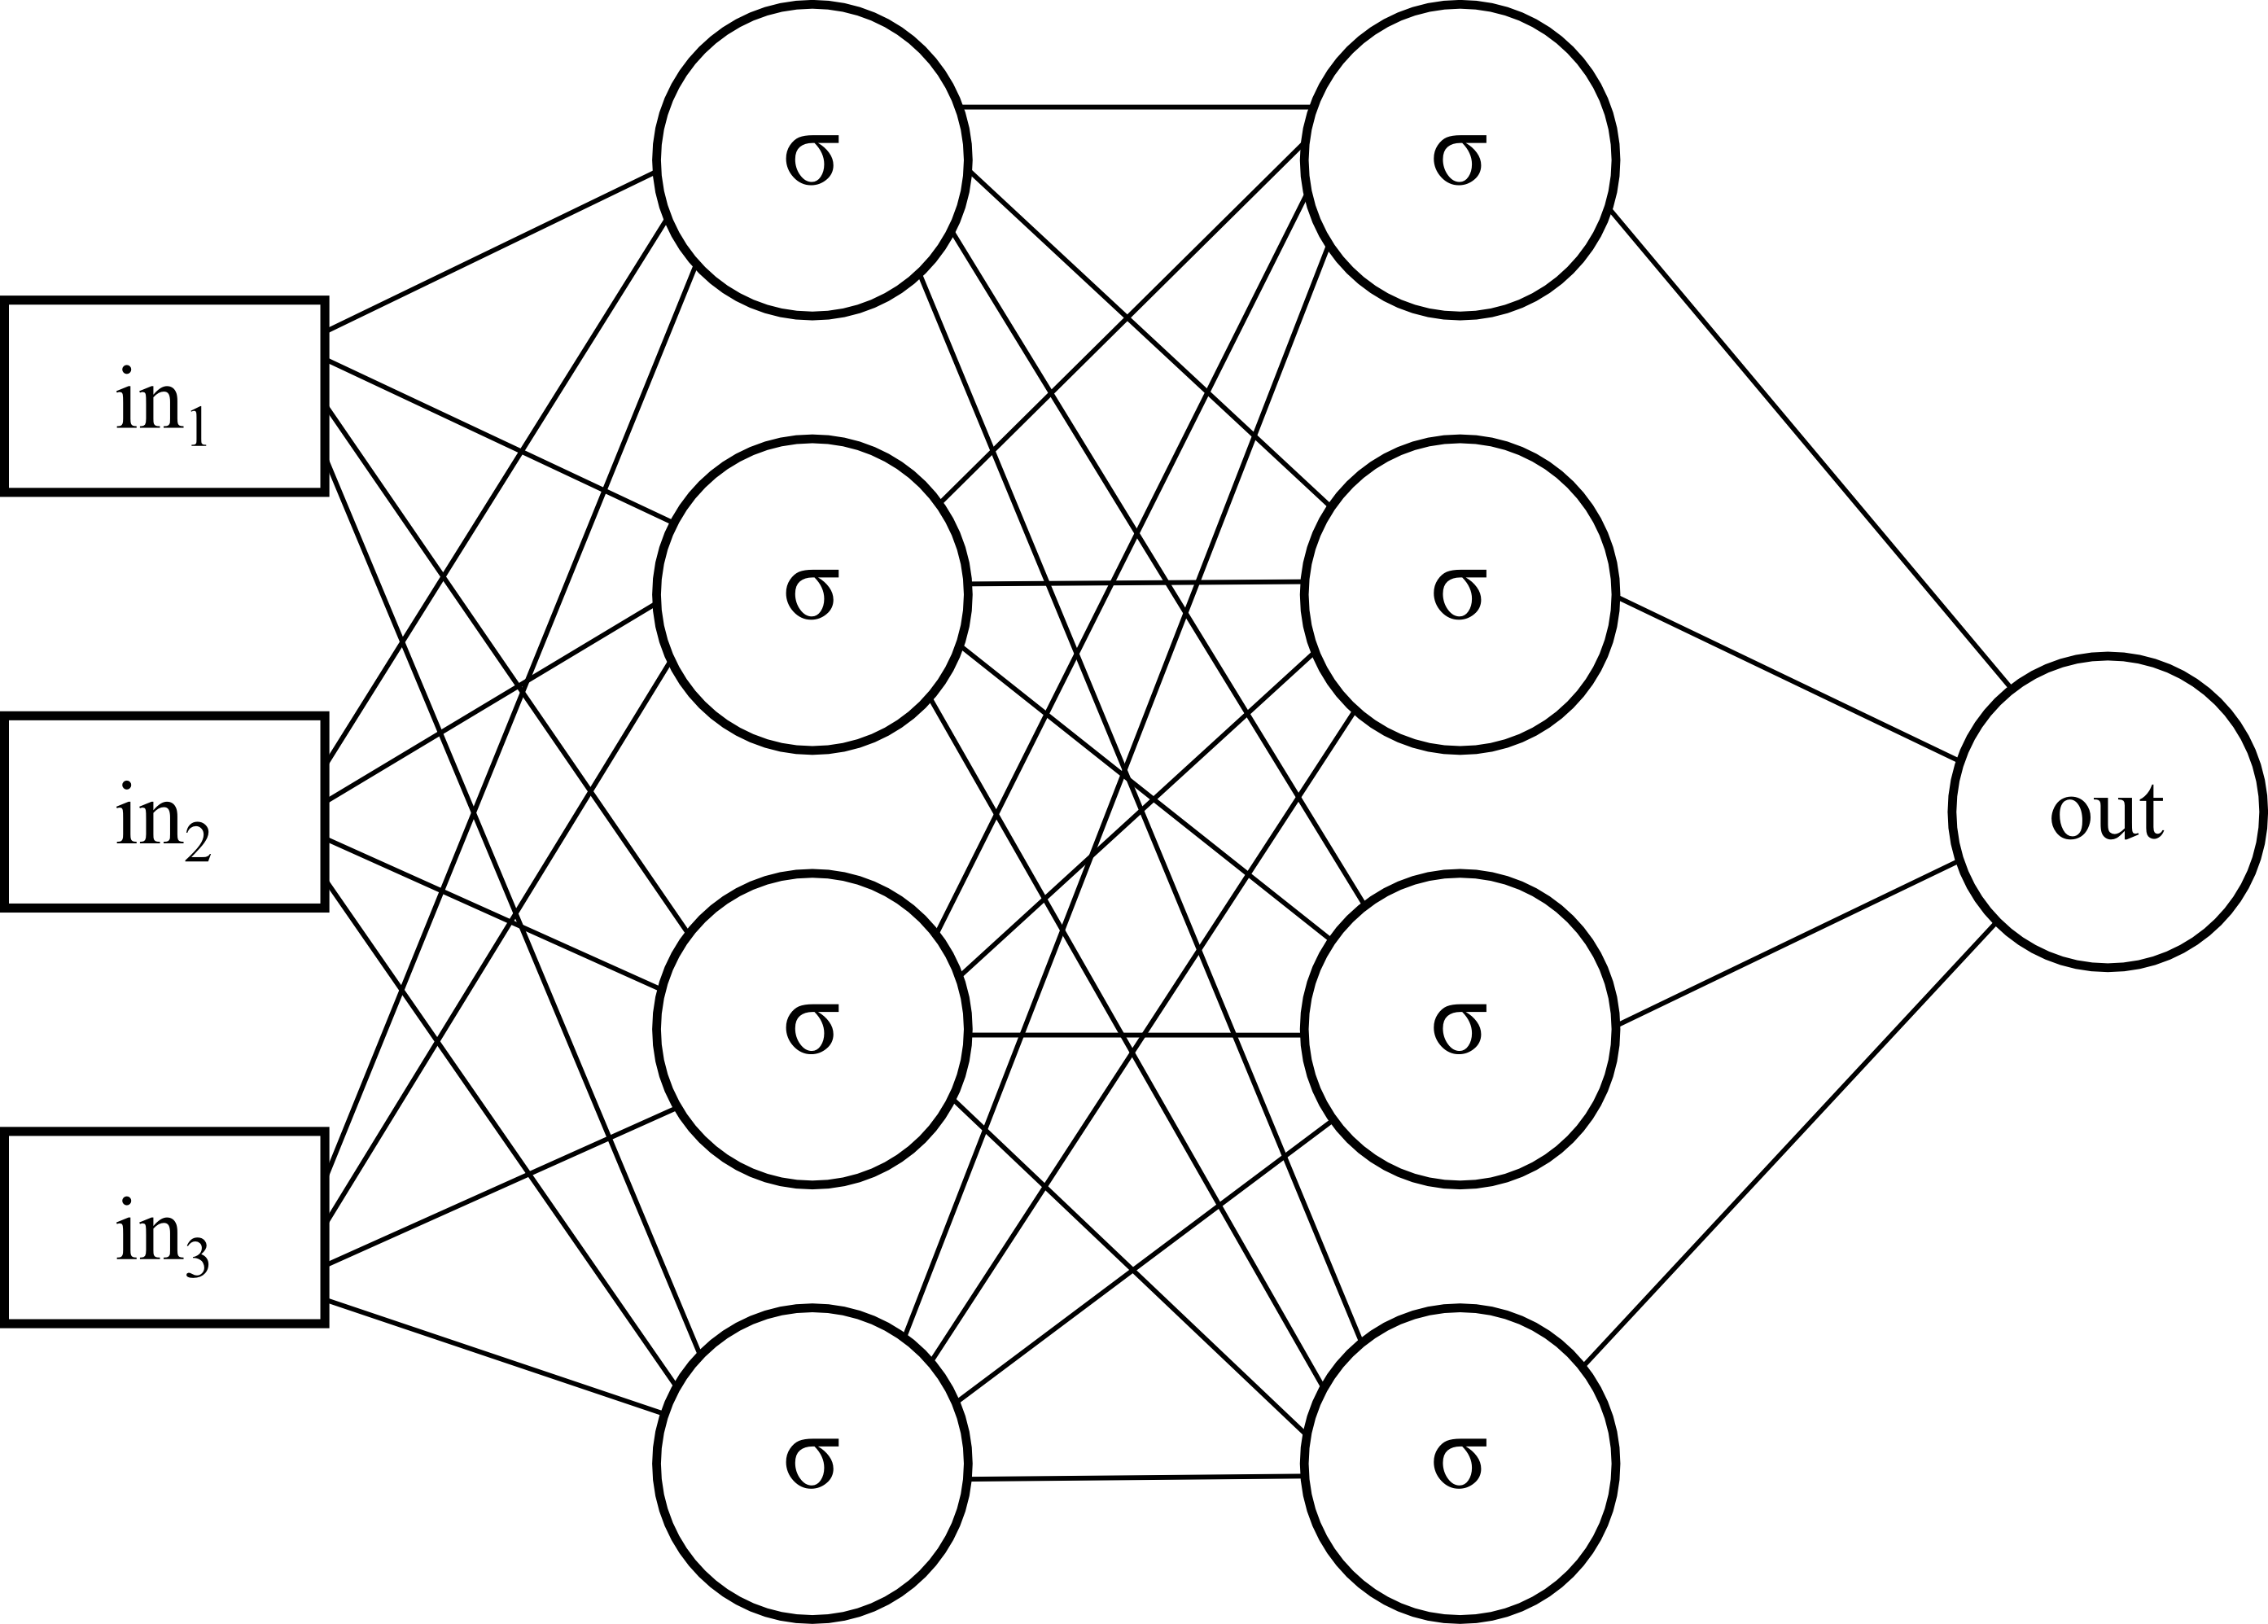
\includegraphics[scale=1]{images/neuron-network.png}
\caption{Ein Neuron}
\label{fig:neuron-network}
\end{figure}

Um aus den einzelnen Neuronen ein Netzwerk zu machen, werden, wie in Abbildung \ref{fig:neuron-layer} Layer gebildet. Ein Layer ist eine Menge an Neuronen, die untereinander nicht direkt verknüpft sind. Layer werden sequenziell hintereinander gehängt, wobei jedes Neuron eines Layers als Eingang für jedes Neuron des jeweils nächsten Layers dient. Ein solches Netzwerk ist auch in Abbildung \ref{fig:neuron-network} zu sehen. Dieses Netzwerk hat einen Layer für die Eingabedaten, einen für die Ausgabedaten und zwei innere Layer. Die inneren Layer werden als von außen Unsichtbar betrachtet und daher auch als Hidden-Layer bezeichnet.

